\documentclass[12pt]{report}

% Packages (keep sorted)
\usepackage{
    algorithm,      % For algorithm environment
    algpseudocode,  % For pseudocode
    hyperref,       % For PDF bookmarks
    tikz,           % For state diagrams
    color,
    listings,
    graphicx
}

\usepackage[margin=0.8in]{geometry}

\definecolor{light-gray}{rgb}{0.9, 0.9, 0.9}
\definecolor{mygreen}{rgb}{0,0.6,0}
\definecolor{mygray}{rgb}{0.5,0.5,0.5}
\definecolor{mymauve}{rgb}{0.58,0,0.82}

\lstset{
    backgroundcolor=\color{light-gray}, % Background color
    basicstyle=\footnotesize,        % the size of the fonts that are used for the code
    belowskip=1pt,
    breakatwhitespace=false,         % sets if automatic breaks should only happen at whitespace
    breaklines=true,                 % sets automatic line breaking
    captionpos=b,                    % sets the caption-position to bottom
    commentstyle=\color{mygreen},    % comment style
    deletekeywords={...},            % if you want to delete keywords from the given language
    escapeinside={\%*}{*)},          % if you want to add LaTeX within your code
    extendedchars=true,              % lets you use non-ASCII characters; for 8-bits encodings only, does not work with UTF-8
    keepspaces=true,                 % keeps spaces in text, useful for keeping indentation of code (possibly needs columns=flexible)
    keywordstyle=\color{blue},       % keyword style
    language=C,                      % the language of the code
    morekeywords={*,...},            % if you want to add more keywords to the set
    numbers=left,                    % where to put the line-numbers; possible values are (none, left, right)
    numbersep=5pt,                   % how far the line-numbers are from the code
    numberstyle=\tiny\color{mygray}, % the style that is used for the line-numbers
    showspaces=false,                % show spaces everywhere adding particular underscores; it overrides 'showstringspaces'
    showstringspaces=false,          % underline spaces within strings only
    showtabs=false,                  % show tabs within strings adding particular underscores
    stepnumber=2,                    % the step between two line-numbers. If it's 1, each line will be numbered
    stringstyle=\color{mymauve},     % string literal style
    tabsize=2,                       % sets default tabsize to 2 spaces
    title=\lstname
}


% State diagrams (i.e. I/O)
\usetikzlibrary{
    shadows,
    positioning,
}
% TODO: move these to another file.
\tikzstyle{block} = [rectangle, draw,
    text width=5em, text centered, rounded corners, minimum height=4em]
\tikzstyle{line} = [draw]
\tikzstyle{cloud} = [draw, rectangle, node distance=3cm,
    minimum height=2em]

% PDF bookmarks setup (keep sorted)
\hypersetup{
    colorlinks=true,
    linkcolor=blue,
}

\begin{document}

% Info section

% TODO come up with something more creative
\title{RTX Project Report}

% TODO check names %
\author{
    Xiang, Dian\\
    20431601\\
    \texttt{dxiang@uwaterloo.ca}
    \and
    Justin McGirr\\
    20413625\\
    \texttt{jmcgirr@uwaterloo.ca}
    \and
    Adrian Cheung\\
    20421743\\
    \texttt{a32cheun@uwaterloo.ca}
    \and
    Aaron Morais\\
    20413440\\
    \texttt{aemorais@uwaterloo.ca}
}

\maketitle

\begin{abstract}
    The AwesomeOS, an real time executable built with Keil Development Environment (Keil IDE) on top of a Keil MCB1700 board with a LPC1768 microcontroller, is implemented as an operating system with basic functionalities and interaction through terminal input / output.

    The operating system offers basic multiprogramming with an API for interprocess communication through many to one message passing with process mailboxes. In addition, it offers the ability for memory management of the heap in the RAM of the board. This lets processes allocate and destroy memory during run time.

    The AwesomeOS also offers services in the form of system processes, which talks to interrupt processes for lower level communication. The first service is a timing service, which lets processes communicate with each other after a delayed period of time. The next service this operating system offers is the ability to interact with users and programmers through keyboard inputs and terminal display outputs. Finally, user processes are able to change and select priorities which determine the order of execution.

    The AwesomeOS tries to offer a fast way to service user processes and finish tasks. It implements a system based scheme which allows other services to be added easily. It also modularizes each section to allow clean maintenance and future extensibility.

\end{abstract}

\tableofcontents
\listofalgorithms
\listoffigures

% Uncomment these if we add any figures or tables
% \listoftables


\part{Introduction}
The software engineering class of 2016 has been given the task of writing a real time executive (RTX) on a Keil MCB1700 board with a LPC1768 microcontroller. This operating provides a basic multiprogramming environment on a uniprocessor core with 5 priority levels, preemption, heap memory management, a basic timing service, and system I/O for user inputs, outputs, and debugging purposes. This report discusses the usage and implementation of this operating system implemented by group 2.

The first section of this report discusses the implementation of the operating system. It discusses the global variables used in the operating system and what their needs are. Then, it goes on to give a layout of each kernel API call that the user has access to. Next, interrupt and system process implementations are discussed in detail. This will cover which API calls use the process and how these processes interact with both the user and the kernel. Example user processes were also written for testing and execution of the operating system. Section \ref{sec:user_processes} goes into more details about each individual user process and what their purpose is in the creation of the operating system. We also discuss the initialization of the OS, which includes parameters the OS is given before its initial execution of a process and the initialization steps it must carry. Finally, we end the kernel API discussion with lessons we have learned and major design decisions that may help other people in the future.

Apart from implementation of the RTX, testing and timing analysis was also done on the operating system. The last section discusses the result of the tests (such as unit tests and debugging techniques) that were done the and results of the timing analysis. The timing analysis analyzes two four kernel API primitives on different machines and with different parameters. The raw material were formalized for analysis using mathematical statistics.



\part{Awesome RTX}
% Make sure to include pseudocode and testing, if appropriate.

\chapter{Global Variables}
\section{Description}
There are various amounts of variables used throughout the RTX. This section describes the global variables that are used to accomplish tasks in the RTX. Other global variables such as the global process IDs can be seen in the appendix (Section \ref{sec:appendix}) There are three major sections that required global variables and data structures: memory management in the heap, scheduler, and user processes.

\section{Heap Data Structures}
The RTX provides functionality to request and release memory from the heap, which is shared and stored in the RAM of the board. There is one main data structure that stores each memory block.

\begin{lstlisting}
typedef struct HeapBlockHeader {
  int source_pid;
  int dest_pid;
  unsigned int send_time;
  struct HeapBlock* p_next;
  struct HeapBlock* p_next_usr;
} HeapBlockHeader;

#define HEAP_BLOCK_SIZE 128

typedef struct HeapBlock {
  HeapBlockHeader header;
  byte            data[HEAP_BLOCK_SIZE];
} HeapBlock;

\end{lstlisting}

The HeapBlock structure stores a header and the content of the block. When a memory is requested, users are given the data with a adjustable size of HEAP\_BLOCK\_SIZE and do not have knowledge of the header. Helper functions in the RTX turn the user block back into kernel block by adjusting the pointer of the block. Each header contains information used for message passing. This global data structure is used in the following sections:
\begin{enumerate}
    \item {\bf Process Message Passing} - Uses this data structure to pass messages between processes. Message envelopes are implemented as HeapBlocks.
    \item {\bf Timer I-Process} - Uses message passing to send delayed messages.
    \item {\bf UART I-Process} - Uses message passing for input and output characters.
    \item {\bf CRT I-Process} - Receives messages and passes message for terminal output.
    \item {\bf KCD Process} - Passes messages to CRT and user processes for display and processing.
\end{enumerate}


\section{Process Scheduler Data Structures}
The RTX has a fixed-priority based scheduler that acts as a uniprocessor system. Context switching is required and the following data structures are used for this purpose.

\subsection{Ready and Blocked Priority Queues}
On initialization, each in memory process is given a process control block (PCB). The PCB contains data on the process such as its process ID, stack pointer, process state, and priority that the kernel will use for scheduling. The blocked and ready priority queues of PCBs keep track of which processes are blocked and ready for execution. Each process is in one of the 5 states at all time listed in ProcessState. Processes that are in state PROCES\_STATE\_READY are on the ready queue. Processes in state PROCESS\_STATE\_BLOCKED are in the blocked queue. There is also a sort of implicit queue for processes blocked on message but we won't go into that in this section.

\begin{lstlisting}
typedef enum {
  PROCESS_STATE_NEW                = 0,
  PROCESS_STATE_READY              = 1,
  PROCESS_STATE_RUNNING            = 2,
  PROCESS_STATE_BLOCKED            = 3,
  PROCESS_STATE_BLOCKED_ON_MESSAGE = 4,
} ProcessState;

typedef struct PCB {
  // Stack pointer
  U32*            sp;

  ProcessID       pid;
  ProcessState    state;
  ProcessPriority priority;

  struct PCB*     p_next;
  // Incoming messages, waiting to be processed.
  HeapBlock*      message_queue;
} PCB;

PCB* g_ready_process_priority_queue[PROCESS_PRIORITY_NUM] = {NULL};
PCB* g_blocked_process_priority_queue[PROCESS_PRIORITY_NUM] = {NULL};
\end{lstlisting}

PCBs and the priority queues are used in the following sections:
\begin{enumerate}
    \item {\bf Memory Management} - When a process requests memory without available memory blocks, the memory management subsystem must add the process to a blocked queue. When a memory block is released, the process with the highest priority in the blocked queue (if any) is moved into the ready queue. Thus, the memory management subsystem must have access to the PCBs, and blocked and ready queues in order to accomplish these task.
    \item {\bf Process Management} - The process management subsystem is the one that schedules processes and keep track of the process priorities. Ready processes are taken from the ready queue to be ran if the current process is blocked or finished its execution. The process management subsystem also takes care of updating the two priority queues when the priority of a process has been changed.
    \item {\bf UART Process} - The UART Process needs access to the PCB. The PCBs also contain a mailbox for messages. The UART displays any incoming messages to the terminal display. Thus, it needs to know the PCB structure in order to gain access to the mailbox.
\end{enumerate}

\subsection{Priorities}
The RTX is based on a fixed-priority scheduler with 4 user process priorities and 3 system process priorities given below. Users are given priorities PROCESS\_PRIORITY\_HIGH to PROCESS\_PRIORITY\_LOWEST. PROCESS\_PRIORITY\_NULL\_PROCESS is given to the null process and PROCESS\_PRIORITY\_SYSTEM\_PROCESS are given to critical processes such as the KCD and CRT. Finally, psuedo-processes, such as the timer I-process and UART I-process are given PROCESS\_PRIORITY\_UNSCHEDULABLE, since they "schedule" themselves whenever an interrupt happens, and should never be run by the normal scheduler (in fact, they don't even have stacks!).

\begin{lstlisting}
typedef enum {
  PROCESS_PRIORITY_INVALID        = 0,
  PROCESS_PRIORITY_SYSTEM_PROCESS = 1,
  PROCESS_PRIORITY_HIGH           = 2,
  PROCESS_PRIORITY_MEDIUM         = 3,
  PROCESS_PRIORITY_LOW            = 4,
  PROCESS_PRIORITY_LOWEST         = 5,
  PROCESS_PRIORITY_NULL_PROCESS   = 6,
  PROCESS_PRIORITY_UNSCHEDULABLE  = 7,

  PROCESS_PRIORITY_NUM            = 8
} ProcessPriority;

typedef enum {
  USER_PROCESS_PRIORITY_HIGH           = 0,
  USER_PROCESS_PRIORITY_MEDIUM         = 1,
  USER_PROCESS_PRIORITY_LOW            = 2,
  USER_PROCESS_PRIORITY_LOWEST         = 3,

  USER_PROCESS_PRIORITY_NUM            = 4,
} UserProcessPriority;
\end{lstlisting}

This priority structure is used by the process management subsystem to schedule and block processes based on their priorities. The RTX provides users with UserProcessPriority while keeping an internal structure of ProcessPriority with additional levels.

\chapter{Kernel API}
% TODO add a section on implementation details and run time analysis.
\section{Description}
This section describes the kernel API that is available to users in the RTX. It will only go into details of how to use each API function call and states of different scenarios. Exact details can be found in the raw code.

\section{Memory Management}
\subsection{Description}
The RTX provides the utility of simple memory management of the heap. The main memory on the Keil MCB1700 is divided into sections of the RTX Image, PCB data, the heap, and process stacks seen in Figure \ref{fig:memory}.

The Keil MCB1700 does not have the necessary hardware to support virtual memory. Thus, a fixed memory management scheme is used. The OS kernel is always loaded into main memory in its entirity. When the OS boots, a user stated number of PCBs and process stack are allocated. The OS also allocates memory for system processes such as the Keyboard Command Decoder Process (KCD) and the CRT Display Process. After allocation of PCBs and process stacks, the remaining memory is used for the heap, which is shared between all processes. This section will be focused on the memory management of the heap.

The heap is further divided into a variable number of blocks. Each block contains a header (HeapBlockHeader) and 128 bytes of data. Depending on the number of user and system processes, the number of available heap memory will vary. The size of the data can vary from 128 bytes but must be set at compile time. The OS supports two kernel calls that gives access to these memory blocks.

\subsection{Requesting Memory}
\label{sec:request_memory}
\begin{lstlisting}
void *request_memory_block();
\end{lstlisting}
\par The first functionality supported by the OS is the ability to request memory. This call gives back a pointer to a memory block in the heap. The size of the memory block is defined by the constant HEAP\_BLOCK\_SIZE, which defaults to 128 bytes. These blocks are used for storing local variables or as envelopes for interprocess communication (described in section \ref{sec:send_message}). The user must cast the memory block to the proper type for his or her own use. An example of the usage is provided below, which stores the numbers 0-31 in an array of size 32.
\begin{lstlisting}
void user_process() {
    int size = 32;

    int* array = (int*)request_memory_block();

    for (int i = 0; i < size; i++) {
        array[i] = i;
    }

    // ...

    release_memory_block((void*)array);
}
\end{lstlisting}
% TODO maybe put a caption here CODE1

\par All processes will share the same heap memory pool. Thus, this primitive will block the process if there are no remaining free memory blocks. In that case, it will only be unblocked there is a new memory block available and if it has the highest priority on the list of processes waiting for a memory block. When using the memory block, the user must be aware of writing past the heap block size. The OS does not check this in any way. Thus, undefined behavior may occur. Also, the user must remember to release the memory block or memory leakage will occur.

\par Requesting memory is reliant on calls to the heap to find an available memory block to allocate. The heap keeps a list of the status of each memory block to determine whether or not a block of memory can be requested. The following is the implementation used by the heap:
\label{fig:findfreeblock}
\begin{algorithm}
  \caption{Requesting Memory}
  \begin{algorithmic}[1]
    \Function{FindFreeBlock}{}
      \For{$i = 0$ to $TotalNumberOfBlocks$}
        \If{FreeSpaceBitmap[i] is a free block}
          \State return i
        \EndIf
      \EndFor
    \State return not found
    \EndFunction
  \end{algorithmic}
\end{algorithm}


The lookup time of the FreeSpaceBitmap is O(1) as it is a simple array lookup and a boolean evaluation. Finding a free block has its dependencies on the total number of blocks. The best case for requesting memory is O(1) when the first block in the heap is free. Since this is a linear search, on average the complexity is O(n) where n is the total number of blocks.

Although this is worse in theta complexity than a simple free-list implementation,
it was chosen because it allows almost all memory errors to be caught immediately,
significantly easing debugging. We verify heap block alignment, check for double-
frees, and verify that the pointer lies within the heap, each of which has helped
us find bugs that would otherwise be invisible while developing the RTX.

\bigskip

\subsection{Releasing Memory}
\begin{lstlisting}
int release_memory_block(void *memory_block);
\end{lstlisting}

\par The second functionality supported by the OS is the ability to release memory. This is a non-blocking (but potentially pre-empting) call that returns the memory block back to the OS. This should be called when a message is received and not passed on or when the process is done using the memory block. If any process is blocked on memory, it will be unblocked and put to the ready queue. If the current process has lower priority than the unblocked process, then the current process will be preempted and the higher priority process will be executed instead. An example of this can be seen in Figure \ref{fig:findfreeblock} on line 13.

\par In order to release the memory, release\_memory\_block will need to rely on the implementation of the heap. As stated in \ref{sec:request_memory}, the heap keeps a list of all available memory blocks. In order to release a memory block, the heap will set that block in the list as a free block. Releasing the block thus has O(1) complexity as it only relies on an array lookup. The implementation is as follows:
\begin{algorithm}
    \caption{Releasing Memory}
    \begin{algorithmic}[1]
    \Function{ReleaseMemory}{MemoryBlock}
      \State FreeSpaceBitmap[position of MemoryBlock] $\gets$ true
    \EndFunction
  \end{algorithmic}
\end{algorithm}


\bigskip

\section{Processor Management}
\begin{lstlisting}
int release_processor();
\end{lstlisting}

\par The OS manages processes as though it is on a uniprocessor. A priority based scheme with context switching is used for scheduling processes. A process can voluntarily release the processor to the OS at any time during its execution. If there are errors in the call, it will return an error without releasing the processor to the OS. If there are no errors and the invoking process is ready to execute, it is put to the end of the ready queue of its priority. If there are no other processes of equal or higher priority, the process will be chosen to execute again. However, if there is, another process will be chosen for execution. Below is an example which prints an increasing number and releases the processor at every turn.

\begin{lstlisting}
void user_process() {
    static num = 0;
    while(1) {
        print(num++);
        release_processor();
    }
}
\end{lstlisting}

\section{Interprocess Communication}
\par Communication between processes is primarilly done through message-based interprocess communication (IPC), although static variables can also be used in some cases. The RTX gives three primitives to carry out this task, one for sending, one for delayed sending, and one for receiving.

\subsection{Send Messages}
\label{sec:send_message}
\begin{lstlisting}
int send_message(int process_id, void *message_envelope);
\end{lstlisting}

\par A process can compose a message envelope to be sent to another process. Memory for envelope message must be requested from the RTX using the request\_memory\_block() routine. The envelope consists of a type (mtype) and the message data (mtext) which must be filled in as seen below. The predefined message types are used for the KCD, CRT, and Wall Clock process, which are built into the RTX. The message data has a predefined size which is smaller than the HEAP\_BLOCK\_SIZE. Thus, any message that are longer will exhibit undefined behavior. The process ID of the receiving process must also be known ahead of time in order to use send\_message().
\newline
\begin{lstlisting}
typedef enum {
    MESSAGE_TYPE_KCD_KEYPRESS_EVENT       = 0,
    MESSAGE_TYPE_KCD_COMMAND_REGISTRATION = 1,
    MESSAGE_TYPE_CRT_DISPLAY_REQUEST      = 2,
    MESSAGE_TYPE_WALL_CLOCK               = 3,
    MESSAGE_TYPE_USER_DEFINED             = 4,

    MESSAGE_TYPE_NUM                      = 5,
} MessageType;

struct msgbuf {
    MessageType mtype;
    char mtext[HEAP_BLOCK_SIZE - sizeof(MessageType)];
};
\end{lstlisting}
\par The primitive returns a status which validates the, message, receiver process ID, and ready queue. User processes is allowed to send a message to any user processes or system processes such as the KCD. If the receiving process is currently blocked on receiving message, this call will add the message to the process' message box and put it back on the message queue. The current process continues to execute unless the receiving process has a higher priority. In that case, the current process will be preempted and put to the back of the ready queue. Thus, this primitive may effect the execution of the process.

\par In order to keep track of messages that have been sent, the messages are stored in a queue, specifically a linked list. Messages are added to the end of the linked list resulting in an O(n) insertion complexity. It is possible to have this run in O(1) time by using a doubly-linked list and keeping track of the first and last elements in the list, but it seemed more important to provide a working prototype first, and optimize the runtime when (if) it became an issue. O(n) is likely to be quite small even in the worst case, given the limited size of the RTX heap.
\newline
\subsection{Receive Messages}
\label{sec:receive_message}
% TODO put labels on sections so we can reference them throughout without worrying about changing numbers

\begin{lstlisting}
void *receive_message(int *sender_id);
\end{lstlisting}
\par A process can use this primitive to receive messages from other processes. Unless the sender\_id is NULL, the sender of the message will be written to the sender\_id parameter. The current process will check its mailbox for any incoming messages. If there are no messages in its mailbox, the routine will block the process and select another process for execution. Execution of the process will occur again if a message is sent from another process and this process has the highest priority in the ready queue. The message\_envelope is heap memory underneath. Thus, it is required that unless the process passes the message onto another process, the final receiving process must release the message\_envelope block after its usage. An example of send\_message and receive\_message is shown below.

\begin{lstlisting}
void process_send() {
    while(1) {
        // Request one block for process_receive to use
        struct msgbuf* message_envelope
            = (struct msgbuf*)request_memory_block();
        message_envelope->mtype = MESSAGE_TYPE_USER_DEFINED_1;
        strcpy(message_envelope->mtext, "process message");
        send_message(PROCESS_RECEIVE_ID, message_envelope);

        // Send another block for process_receive to send to CRT
        struct msgbuf* message_envelope
            = (struct msgbuf*)request_memory_block();
        message_envelope->mtype = MESSAGE_TYPE_USER_DEFINED_2;
        strcpy(message_envelope->mtext, "print this");
        send_message(PROCESS_RECEIVE_ID, message_envelope);
    }
}

void process_receive() {
    while(1) {
        struct msgbuf* message
            = (struct msgbuf*)receive_message(NULL);
        if( message->mtype = MESSAGE_TYPE_USER_DEFINED_2 ) {
            // Send to CRT for printing; do not release memory
            message->mtype = MESSAGE_TYPE_CRT_DISPLAY_REQUEST;
            send_message(PROCESS_ID_CRT, message);
        } else {
            // Do something with the message then release it
            release_memory_block( (void*)message );
        }
    }
}
\end{lstlisting}

\subsection{Delayed Messages}
\begin{lstlisting}
int delayed_send(int process_id, void *message_envelope, int delay);
\end{lstlisting}

\par This primitive is very similar to the primitive of send\_message in section \ref{sec:send_message} with the addition of a delay. Instead of sending the message immediately, the message will be sent delay number of milliseconds. The message\_envelope is constructed in the same way. The process\_id will be the receiving process. The execution of the process may be preempted after a the delay period if the receiving process was blocked on receive\_message and has a higher priority.

\section{Process Priority}
\par The RTX schedules processes based on a fixed priority scheme. Thus, the RTX provides the utility to change priorities and to get the process priority of any user processes.

\subsection{Set Process Priority}
\label{sec:set_process_priority}
\begin{lstlisting}
int set_process_priority(int process_id, int priority);
\end{lstlisting}

This primitive allows user processes to set the priorities of other user processes. User processes are not allowed to set the priorities of any system processes. System processes, however, are allowed to set the priorities of other system or i-processes. The primitive validates if the current process is allowed to set the priority of the process with process\_id and whether it's a valid process\_id. It also checks the validity of the priority. An error status of RTX\_ERR is given back if the validation does not pass. If properly set, a status of RTX\_OK is returned. The caller of this primitive is not blocked but can be preempted if the priority of the set process is higher. Otherwise, the process continues to execute. An example usage is shown in section \ref{sec:get_process_priority}

\bigskip

\subsection{Get Process Priority}
\label{sec:get_process_priority}
\begin{lstlisting}
int get_process_priority(int process_id);
\end{lstlisting}
Given a process\_id, this primitive gives back the priority of any processes including any system or i-processes to a user process. A invalid process\_id will result in a RTX\_ERR status. Otherwise, a RTX\_OK is returned to the caller. An example usage of both get and set process priority is shown below.

\begin{lstlisting}
// Assume this process has a process ID of 3
// and there is another user process with ID of 1
void user_process() {
    int process_priority_3 = get_process_priority(3);
    if( process_priority_3 == USER_PROCESS_PRIORITY_MEDIUM ) {
        // Make process 1 have a higher priority
        // This call will preempt
        int status = set_process_priority(
                        1, USER_PROCESS_PRIORITY_HIGH );
        if( status == RTX_ERR ) {
            release_processor();
        }
    }
}
\end{lstlisting}


\chapter{Interrupts and Their Handler and Processes}
The operating system supports two interrupt processes, a timer I-process and a UART I-process.
\section{Timer I-Process}
At initialization of the OS, we initialize prescale registered to have a value of 12499, which equals 1 millisecond along with other values that require the interrupt to occur. With these initialized values, we enable the timer 0 interrupts for every 1 millisecond. Once an interrupt occurs, the following handler handles the interrupt.

\begin{algorithm}
    \caption{Timer Interrupt}
    \begin{algorithmic}[1]
      \Function{TIMER0\_IRQHandler}{}
          \State Disable other interrupts
          \State Save state
          \State \Call{c\_TIMER0\_IRQHandler}{}
          \State Enable other interrupts
          \State Put state back and go back to original execution
      \EndFunction
      \bigskip
      \Function{c\_TIMER0\_IRQHandler}{}
          \State Reset interrupt bit
          \State Increase static timer count
          \State message\_peek = \Call{sorted\_message\_queue\_top}{}
          \If{message\_peek time has elapsed}
              \State message = \Call{sorted\_message\_queue\_pop}{}
              \State \Call{send\_message}{message}
              \State \Call{preempt\_if\_necessary}{}
          \EndIf
      \EndFunction
  \end{algorithmic}
\end{algorithm}
The interrupt process is used to keep a timer accurate to 1 millisecond. It is also used for the delayed send primitive in the kernel API. Messages sent to the timer process are kept in a special mailbox that sorts the messages by earliest send time. On each interrupt, the handler checks whether there are message that have elapsed their delay time and sends them. It preempts the current process if a process is blocked on receive and has a higher priority than the currently interrupted process or running process. Interrupts are also disabled from the start and end of this routine. This is to prevent interrupt nesting to occur. If another interrupt occurs in the middle of this interrupt routine, it will be processed after the routine is finished.

\section{UART I-Process}
The UART I-Process is the center of receiving keyboard input and transmitting characters for output.

\subsection{Input}
\label{sec:uart_input}
The first task of the UART is to receive keyboard input. We receive one input character for each interrupt. This character is passed in the form of a message to the KCD for processing, where it will output to the CRT and be processed for any incoming commands. The input section of the UART also handles debugging hot keys. Three character hot keys: 'a', 'b', 'c', and 'd' are chosen to output the ready queue, blocked on resource queue, blocked on message queue, and timer delayed message queue respectively. These outputs use the polling output rather than the interrupt output because if memory was to run out during execution, we still want to see the output of the queues. This cannot be done with interrupts as it requires message passing, thus memory allocation.

\begin{algorithm}
    \caption{UART Input}
    \begin{algorithmic}[1]
      \If{keyboard input interrupt}
          \State char\_in = input\_character
          \If{char\_in is 'a' }
              \Call{print\_ready\_queue}{}
          \ElsIf{char\_in is 'b' }
              \Call{print\_blocked\_memory\_queue}{}
          \ElsIf{char\_in is 'c' }
              \Call{print\_blocked\_receive\_queue}{}
          \ElsIf{char\_in is 'd' }
              \Call{timer\_print\_delayed\_message\_queue}{}
          \EndIf
          \State message = \Call{allocate\_memory\_for\_message}{}
          \State message.Type = MESSAGE\_TYPE\_KCD\_KEYPRESS\_EVENT
          \State message.Data = char\_in
          \State \Call{send\_message}{message}
      \EndIf
  \end{algorithmic}
\end{algorithm}

\subsection{Output}
\label{sec:uart_output}
The second task of the UART is to output characters onto terminal display. A message can contain up to 20 characters. However, the UART display interrupt only supports one character output per interrupt. Thus, the interrupt bit is enabled for the message and a message buffer counter is increased every time an interrupt occurs until the entire message has been outputted to the terminal character by character. Putting this together, we have the following implementation.

\begin{algorithm}
    \caption{UART Output}
    \begin{algorithmic}[1]
      \If{keyboard output interrupt}
          \If{there is no more characters in the message to print}
              \State \Call{memory\_release\_block}{message}
              \State turn off output interrupt bits
          \Else
              \State char\_out = message->Data[count]
              \State give char\_out to register for output
              \State count++
          \EndIf
      \EndIf
  \end{algorithmic}
\end{algorithm}


\subsection{Putting it together}
The UART's interrupt handler handles both input from the keyboard and output to terminal screen. Thus, the overall handler has this implementation:

\begin{algorithm}
    \caption{UART Interrupt}
    \begin{algorithmic}[1]
      \Function{UART0\_IRQHandler}{}
          \State Disable other interrupts
          \State Save state
          \State \Call{c\_UART0\_IRQHandler}{}
          \State Enable other interrupts
          \State Put state back and go back to original execution
      \EndFunction
      \bigskip
      \Function{c\_UART0\_IRQHandler}{}
          \If{input}
              \State run code from section \ref{sec:uart_input}
          \ElsIf{output}
              \State run code from section \ref{sec:uart_output}
          \Else
              \State error
          \EndIf
      \EndFunction
  \end{algorithmic}
\end{algorithm}

Similar to the timer I-process, the UART I-process will preempt the current process if another process with higher priority receives its message after being blocked on receive. The UART I-process also does not support nested interrupts. Other interrupts are disabled during this routine and will occur only after this handler has finished its execution.

% TODO Make sure to include pseudo-code and testing, if appropriate.

\chapter{System and User Processes}

\section{System Processes}
\subsection{Description}
The RTX consists of system processes that sit on top of the kernel. These system processes usually have higher priority than user processes because they carry out tasks for the OS that the kernel cannot do otherwise. System processes in this RTX includes the null process, and I/O processes.

\subsection{Null Process}
The design of the RTX requires that a process should always be executing. Thus, if there are no user or other system processes, the null process executes. The only job of the null process is to keep the processor running. It has the lowest priority of any process using the RTX. If any process is added into the ready queue during the execution of this process, a preemption will occur and the new process will take control of the processor. The final implementation follows the following form.

\begin{algorithm}
    \caption{Null Process}
    \begin{algorithmic}[1]
      \Function{null\_process}{}
        \While{true}
        \EndWhile
      \EndFunction
    \end{algorithmic}
\end{algorithm}


\subsection{CRT Display Process}
\label{sec:crt_process}
% TODO make footnotes for details
The RTX supports output to terminal display. CRT is a system process that the RTX uses to accomplish the task of display. The CRT process depends on the UART I-Process (details of the UART can be found in Section \ref{sec:uart_output}). The CRT is implemented using the following algorithm.

\begin{algorithm}
  \caption{CRT}
  \begin{algorithmic}[1]
    \Function{crt\_process}{}
      \While{true}
          \State message = \Call{receive\_message}{NULL}
          \If{message is not a CRT display request}
              \State continue
          \EndIf
          \State \Call{send\_message}{PROCESS\_ID\_UART, message}
          \State Set interrupt bits
      \EndWhile
    \EndFunction
  \end{algorithmic}
\end{algorithm}

 The CRT display process accepts message requests from any process of type MESSAGE\_TYPE\_CRT\_DISPLAY\_REQUEST. This tells the CRT to send the message for display to the UART I-process, which interacts with the hardware registers to output to terminal. Since the UART process is an interrupt process, the interrupt bit must be set in order for the process to run. Thus, after sending the message to UART's mailbox, the CRT process enables the interrupt bits for the I-process to trigger. The UART I-process passes the message character by character to the hardware to display to the terminal.

\subsection{Keyboard Command Decoder Process}
\label{sec:kcd_process}
The RTX provides functionality to forward user input commands to a particular process. The keyboard command decoder process (KCD) handles two tasks: giving input to the CRT for terminal display and forwarding certain inputs to different processes for further processing. For the first task, all keyboard inputs are filtered by the KCD. The UART I-process is called when a key is first pressed. The UART I-process (explained further in section \ref{sec:uart_input}) then passes a message to the KCD telling of type key press. In the first case, the KCD will take this message and pass it on to the CRT for terminal display.

In the latter case, processes can register a command with the KCD. Each command registration consists of a single capital letter of the alphabet. If a command is taken, the KCD will not register the command and exit with an error. After a valid command has been registered, user input with the pattern "\%" followed by a upper case character will be parsed by the KCD. If user types in "\%" followed by a registered character, the KCD will buffer the input until the user presses the return key. In that scenario, the KCD will pass it onto the registered process. The following algorithm of the KCD explains this in more detail.

\begin{algorithm}
  \caption{KCD}
  \begin{algorithmic}[1]
    \Function{process\_input}{message}
        \If{ There a "\%" character in the buffer }
            \If{message.Content is a command character}
                \State add to buffer
            \Else
                \State clear buffer
            \EndIf
        \ElsIf{ message.Content is "\%" }
            \State add to buffer
        \ElsIf{ message.Content is enter and buffer is not empty}
            \State send buffer to registered command
        \EndIf
        \State Send message to CRT to display

    \EndFunction

    \bigskip

    \Function{process\_register}{message}
        \If{ message.Command has not been taken}
            \State register message.Command
        \Else
            \State error
        \EndIf
    \EndFunction

    \bigskip

    \Function{kcd\_process}{}
        \State initialization
        \While{true}
            \State message = \Call{receive\_message}{NULL}
            \If{message type is key press input}
                \State \Call{process\_input}{message}
            \ElsIf {message type is command registration}
                \State \Call{process\_register}{message}
            \EndIf
        \EndWhile
    \EndFunction
  \end{algorithmic}
\end{algorithm}

An example of this usage is the wall clock process (described in more detail in section \ref{sec:wall_clock_process}). The wall clock process registers the character 'W' as a command. The registration will be done by passing a message to the KCD of command registration type. This message is received by the KCD. If the 'W' command has not been registered, it becomes registered by the wall clock process. Meanwhile, the user types in random characters. Any character that is not '\%' is passed by the KCD to the CRT for display. Once a '\%' is received, the KCD checks the next character to see if it's a registered command. If its not a registered command, the KCD clears the buffer and starts at the beginning. If it is a registered command, the KCD keeps a buffer of all the input characters. This buffer fills with data and is sent to the wall clock process for processing after the user presses enter. The buffer is only 20 characters long. Thus, any data for a process after 20 characters will not be sent to the registered process on enter.

\section{User Processes}
\label{sec:user_processes}

\subsection{Description}
The RTX contains user processes that operate at an unprivileged level. These processes are designed to demonstrate the overall functionality of the system. Tasks are carried out within these processes by making calls to the RTX APIs, taking advantage of the kernel abstraction to accomplish more user specific goals. User processes include the test processes, wall clock process, set priority command process and stress test processes.


\subsection{User-Level Test Processes}
The user-level test processes were designed to test the RTX. Six aspects of the RTX’s functionality was chosen to be tested through the RTX API. Without using any knowledge of the kernels design or data structures, the following functionality was tested within 6 processes:
\newline
\noindent{{\bf Test Process 1 - }Request Memory and Release Memory}

\noindent The first test process tests the functionality of requesting and releasing memory blocks. A number of memory blocks are requested and stored sequentially, and then immediately released. The process is implemented using the following algorithm.
\begin{algorithm}
  \caption{User Test Process 1}
  \begin{algorithmic}[1]
    \Function{TEST\_PROCESS\_1}{}
      \State number\_of\_memory\_blocks = 30
        \For{i = 0 to number\_of\_memory\_blocks}
        \State memory\_blocks[i] = REQUEST\_MEMORY\_BLOCK()
      \EndFor
      \State mark the request memory test as passed
      \For{i = 0 to number\_of\_memory\_blocks}
        \State RELEASE\_MEMORY\_BLOCK(memory\_blocks[i])
      \EndFor
      \State mark the release memory test as passed
      \State set the priority of process 1 to lowest
      \State set the priority of process 2 to high
      \While{true}
        \State increment static iteration counter
      \EndWhile
    \EndFunction
  \end{algorithmic}
\end{algorithm}

\noindent {\bf Test Process 2 - }Set priority

\noindent The second test process tests the functionality of setting the priority of processes. In addition, the process preemption that can occur due to changing priorities is also tested. During this test, process 3 and 4 are given higher priority than process 2. Once this occurs, process 2 is preempted and is not scheduled to run again. Details of this process are shown in the following algorithm.
\begin{algorithm}
  \caption{User Test Process 2}
  \begin{algorithmic}[1]
    \Function{TEST\_PROCESS\_2}{}
      \State mark the set priority test as passed
      \State set the priority of process 3 to high
      \State set the priority of process 4 to medium
      \State set the priority of process 2 to lowest

      \State mark the set priority test as failed
      \While{true}
      \EndWhile
    \EndFunction
  \end{algorithmic}
\end{algorithm}

\noindent {\bf Test Process 3 and 4 - }Send and receive message

\noindent Process 3 and 4 test the send and receive message functionality by sending messages between each other. Process 3 waits to receive messages from process 4. Once process 3 has received a set number of messages and process 4 has sent the same required number, the test will be marked as successful. The next test will be conducted by increasing the priority of process 5 and decreasing the priorities of process 3 and 4 to trigger preemption. The details of these two test processes can be seen below.
\begin{algorithm}
  \caption{User Test Process 3 and 4}
  \begin{algorithmic}[1]
    \Function{TEST\_PROCESS\_3}{}
      \State received\_messages = 0
      \State required\_messages = 50
      \While{true}
        \State mark received message test as failed
        \State message = RECEIVE\_MESSAGE(NULL)
        \State received\_messages = received\_message + 1
        \State RELEASE\_MEMORY\_BLOCK(message)
        \If{received\_messages is equal to required\_messages}
          \State mark the receive message test as passed
              \State set the priority of process 5 to high
              \State set the priority of process 4 to lowest
              \State set the priority of process 3 to lowest
        \EndIf
      \EndWhile
    \EndFunction

    \Function{TEST\_PROCESS\_4}{}
      \State sent\_messages = 0
      \State required\_messages = 50
      \State test\_phrase = "The quick brown fox jumped over the lazy dog”
      \While{true}
        \State message\_envelope = REQUEST\_MEMORY\_BLOCK()
        \State set the value of mtype property for message\_envelope to 10
        \State set the value of mtext property for message\_envelope to test\_phrase
        \State sent\_messages = sent\_message + 1
        \If{sent\_messages is equal to required\_messages}
          \State mark the send message test as passed
        \Else
          \State send message\_envelope to process 3
        \EndIf
      \EndWhile
    \EndFunction
  \end{algorithmic}
\end{algorithm}

\noindent {\bf Test Process 5 - } Delayed send

\noindent Process 5 tests the delayed send functionality of the RTX. To begin this test, the process sends a message to itself. Immediately afterward a receive message api call is made, blocking the process. Process 1 is at medium priority and runs during the 1000 ms duration that process 5 is blocked. By incrementing a static pointer in a while loop within process 1, verifying that the counter is greater than 0 confirms that the message sent successfully and in a delayed manner as desired.  The delayed send process algorithm can be seen below.

\begin{algorithm}
  \caption{User Test Process 5}
  \begin{algorithmic}[1]
    \Function{TEST\_PROCESS\_5}{}
      \State set\_process\_priority(1, USER\_PROCESS\_PRIORITY\_MEDIUM)

      \State message\_envelope = REQUEST\_MEMORY\_BLOCK()
      \State send message\_envelope to process 5 in 1000 ms
      \State message = RECEIVE\_MESSAGE(NULL)

      \If{static iteration counter is greater than 0}
        \State mark the delayed send test as passed
      \EndIf
      \State RELEASE\_MEMORY\_BLOCK(message)

      \State set the priority of process 1 to lowest
      \State set the priority of process 5 to lowest
      \State set the priority of process 6 to high
      \While{true}
      \EndWhile
    \EndFunction
  \end{algorithmic}
\end{algorithm}

\subsection{Wall Clock Process}
\label{sec:wall_clock_process}
    The RTX provides a process that will act as a wall clock. When it is running, it will output its current time value to the CRT each second. The wall clock registers for commands with the KCD and based on commands that it is given, the wall clock can be started at time “00:00:00”, set to a user specified time or terminated.

  The wall clock registers the character ‘W’ with the KCD process. A reset, set or terminate command can be issued to the wall clock process. If a reset command is received, the process will begin updating the time every second starting from “00:00:00” to the console CRT. When a set command is received, the input is parsed, verified for correctness and then the wall clock begins outputting the clock every second starting from the user supplied time. A terminate command stops the console out from occurring.

  In order for the wall clock to output to the console each second, it sends a message to itself with a one second delay. If a message of this nature is received by the process, it will compute the current time offset based on the time elapsed value from the timer interrupt handler. With this time offset, it will print the current time. The implementation details can be found in algorithm 14.

\begin{algorithm}
\label{alg:wall_clock}
  \caption{Wall Clock}
  \begin{algorithmic}[1]
    \Function{wall\_clock\_process}{}
      \State is\_running = false
      \State time\_base = 0
      \State register the character ‘W’ as a command with the KCD process.
      \State send a message of type MESSAGE\_TYPE\_WALL\_CLOCK to this process in 1000ms
      \While{true}
        \State message = RECEIVE\_MESSAGE(NULL)
        \If{message is empty}
          \State log error
          \State continue while loop
        \EndIf
        \If{message property mtext is clock reset}
          \State is\_running = true
          \State time\_base = 0 - TIMER\_ELAPSED\_MS()
          \State RELEASE\_MEMORY\_BLOCK(message)
          \State break while loop
        \ElsIf {message property mtext is clock set}
          \State new\_time\_offset = wall\_clock\_parse\_time(message property mtext)
          \If{new\_time\_offset is less than zero}
            \State is\_running = false
            \State set message property mtype to MESSAGE\_TYPE\_CRT\_DISPLAY\_REQUEST
            \State send message to the CRT process
            \State continue while loop
          \EndIf
          \State is\_running = true
          \State time\_base = new\_time\_offset - TIMER\_ELAPSED\_MS()
          \State RELEASE\_MEMORY\_BLOCK(message)
          \State break while loop
        \ElsIf{message property mtext is clock terminate}
          \State is\_running = not value of is\_running
                \State RELEASE\_MEMORY\_BLOCK(message)
                \State break while loop
        \Else
          \If{message mtype is not of type wall clock}
            \State log error
            \State RELEASE\_MEMORY\_BLOCK(message)
            \State continue while loop
          \EndIf
          \State timer\_message = REQUEST\_MEMORY\_BLOCK()
          \State set timer\_message mtype to MESSAGE\_TYPE\_WALL\_CLOCK
    send timer\_message to wall clock in 1000ms
          \If{if is\_running}
            \State set message mtype to MESSAGE\_TYPE\_CRT\_DISPLAY\_REQUEST
            \State set message mtext to value from function wall\_clock\_print\_time given (TIMER\_ELAPSED\_MS() + time\_base)
            \State send message to the CRT process
          \Else
            \State RELEASE\_MEMORY\_BLOCK(message)
          \EndIf
          \State break while loop
        \EndIf
      \EndWhile
    \EndFunction
  \end{algorithmic}
\end{algorithm}


\subsection{Set Priority Command Process}
  The RTX provides users with the ability to set the priority of other user processes via KCD commands. The set priority command process registers the character ‘C’ as a command with the KCD. The expected input command input looks like “\%C process\_id new\_priority”. The user can specify the process id of any user process and apply a new priority within the accepted range for user processes. The process functions by waiting to receive commands from the KCD, parsing a received command and taking action on the command inputed. Taking action involves using the set\_process\_priority function from the RTX api and the priority change occurs immediately, potentially causing preemption to occur.

\subsection{Stress Test Processes}
The RTX contains three stress test processes designed to work with each other to verify the behavior of the system. By depleting the available memory blocks of the system, the stress tests processes A, B and C test the robustness of the system by verifying correctness of behavior under heavy load. This heavy load on the system would generally never be tested with regular user processes. When the memory blocks are depleted, certain functionality of the system such as hot key debugging services within the uart must be made available. Additionally, as the memory stress is decreased, the memory blocks must be distributed appropriately to the highest priority process. Through stress testing our system, we were able to determine areas of weakness and make our RTX more robust.

\chapter{Initialization}

\section{Initialization Parameters}
The RTX has several initialization parameters that have defaults but can be tuned to the users requests. The following are parameters that can be given to the OS before it boots
\begin{enumerate}
    \item { \bf Heap block size }- The memory block size determines the size of each block in the heap. This variable is initially defined as 128 bytes. However, it can be tuned by changing HEAP\_BLOCK\_SIZE define.
\begin{lstlisting}
#define HEAP_BLOCK_SIZE 128
\end{lstlisting}

    \item { \bf Message Types }- User processes that require special message types can add their own defined types into the OS defined list of message types. The default is the following.
\begin{lstlisting}
typedef enum {
    MESSAGE_TYPE_KCD_KEYPRESS_EVENT       = 0,
    MESSAGE_TYPE_KCD_COMMAND_REGISTRATION = 1,
    MESSAGE_TYPE_CRT_DISPLAY_REQUEST      = 2,
    MESSAGE_TYPE_WALL_CLOCK               = 3,
    MESSAGE_TYPE_USER_DEFINED             = 4,

    MESSAGE_TYPE_NUM                      = 5,
} MessageType;
\end{lstlisting}

    \item { \bf Number of Processes }- The number of processes must be stated at the beginning by the user or users. The default number is 6 indicating the 6 test user processes in place. A user can add or remove process routines and vary the number of processes by the following define:
\begin{lstlisting}
#define NUM_TEST_PROCS 6
\end{lstlisting}

    \item { \bf Process Initialization Variables }- Each process has a set of initialization variables it can change before the process is added for execution in the operating system. All of the variables are defined and can be changed in the PROC\_INIT structure.
\begin{lstlisting}
typedef enum {
    USER_PROCESS_PRIORITY_HIGH           = 0,
    USER_PROCESS_PRIORITY_MEDIUM         = 1,
    USER_PROCESS_PRIORITY_LOW            = 2,
    USER_PROCESS_PRIORITY_LOWEST         = 3,

    USER_PROCESS_PRIORITY_NUM            = 4,
} UserProcessPriority;

typedef struct {
    int pid;
    UserProcessPriority priority:32;
    int stack_size;
    void (*entry_point) ();
} PROC_INIT;
\end{lstlisting}
        \begin{enumerate}
            \item { \bf Process ID (pid) }- Each process is assigned a particular process ID as long as two processes does not have the same ID.
            \item { \bf Process Priority (priority) }- Each process is assigned a priority from lowest to high.
            \item { \bf Process Stack Size (stack\_size) }- Each process is assigned a default value of 512 bytes for the stack size. This value can be varied if a user process wants more stack and this number is known at the beginning
            \item { \bf Process Entry Point (entry\_point) }- Location of initial instructions.
        \end{enumerate}
\end{enumerate}

\section{Initialization Steps}
After setting up the initial parameters, the OS takes several steps to boot.

\begin{enumerate}
    \item Initializes terminal 2, also known as UART1, for display output using polling method. This is used for debugging purposes of the OS.
    \item Initialize terminal 1, also known as UART0, for display output using interrupts. This serves as the main display of keyboard input, wall clock output, and any KCD registered commands.
    \item Initialize main memory for the OS and processes. Figure \ref{fig:memory} shows the final memory layout. Let's assume we have n processes.
        \begin{enumerate}
            \item Initialize the start pointer to the end of the RTX image with padding
            \item Initialize the end pointer to the end of RAM
            \item Allocate PCB block for each process totaling to n PCB blocks
            \item Allocate stack block for each process given the stack size
            \item Separate remaining memory between the PCB and process stacks into heap blocks.
        \end{enumerate}
    \item Initialize registers for timer interrupts
    \item Hand the processor over to the first process and start the initial execution.
\end{enumerate}

\chapter{Major Design Changes}

\section{Description}

\section{Heap}
One of the more significant design changes we had to do in our RTX was to add a
header to all blocks in our heap, in order to support sending arbitrary heap
blocks to arbitrary processes, while allowing the user code to still use the
entire allocated block. This header contained information usable only within the
kernel itself, currently just for message passing, although it could theoretically
be used for other purposes as well. As part of this change, we had to ensure that
all kernel-level functions passed around HeapBlocks (i.e. a pointer to the
address before the heap block's header), while all of the user-facing functions
passed around a pointer to the HeapBlock's data section (otherwise the user
process would end up overwriting the kernel's data structures inadvertedly).
Fortunately, this wasn't a huge change to implement since a limited number of
subsystems relied on the heap functionality at the time, but it took quite a bit
of debate and discussion to decide on this solution, and accidentially came back
to bite us in P3 where we forgot to translate a user heap block pointer into
a kernel heap block pointer before passing it to a kernel-level function.

If I were to do it again, I would probably opt for a footer as opposed to a
header. This would have allowed us to keep the user-level and kernel-level
pointers the same, avoiding any possibility of translation errors. But alas,
this solution didn't even occur to me (nor anyone in our group) at the time.
\section{Scheduler}

\section{Lessons Learned}
  Over the course of this RTX project, we faced many obstacles. As we overcame each obstacle, we were able to identify the mistakes we had made and learn from them. The lessons learned from our mistakes allowed us to work more and more effectively, avoiding previous pitfalls that cost us a fair amount of development time.

The successful implementation of the RTX project can be mainly attributed to the fact that the development process of the project was well defined early on. We were highly organized from the outset, defining coding conventions for the project, enforcing code reviews for code that wasn’t pair programmed and creating a private github repository. This repository provided us with a distributed version control system so that group members could contribute code from their own machines. Additionally, we were able to use the issue tracking and code review functionality available within github to keep our project organized.

Time management was an issue that plagued development. For most deliverables, a considerable amount of work was done right before the deadline. If we had managed our time better, the code quality of the system could potentially be better, there would have been less stress to meet deadlines and additional functionality such as memory protection could have been implemented for the RTX.

There were some mistakes that we ran into often when working on this project. When variables are not initialized, this mistake is difficult to find. Using the simulator within the Keil IDE does not reveal this issue because the simulator sets all variables to empty values on creation. However, when testing on the board, values would instantiated with garbage value causing issues. Additionally, not clearing the values in memory blocks caused issues when they were reallocated for reuse. For example, an element was able to point back to itself because the header was not cleared. Conducting development of the RTX while testing on the board and being more cautious avoided mistakes such as this.

For debugging, the use of unit tests and a hard fault handler was extremely useful. Unit tests were written for simple functions and data structures such as our priority queue, heap queue and heap. Testing these functions provided a sanity check of the systems functionality and verified that changes did not cause any regressions. The hard fault handler was also extremely useful for tracking down bugs. It provided access to memory at the time of hard fault, including the program counter, making it easier to pinpoint specific issues with the system.

Overall, we are happy with what we have accomplished. We’ve created a robust system that meets all of the design criteria.

\part{Testing and Analysis}

\chapter{Testing}

\section{Description}

In order to test the operating system there were 3 main methods of testing: Unit Tests, Testing Processes, and Manual Testing. The latter was used for the CRT and KCD. Unit tests were implemented for the various data structures in the operating system. For the different queues that were implemented, the unit tests do basic logic tests, checking the push and pop functionalities in increasingly complex senarios. The heap was also unit tested. In this case there were unit tests in place to validate expected behaviour for memory blocks being continuously freed, validation for misaligned memory, freeing invalid blocks, and double freeing. All unit tests set up a specific state, called a specific method, and had its results verified against the expected. This helped us catch more than a few stupid bugs (such as forgetting to return a value), and a fair share of tricky ones (such as not handling adding a block that already has a next pointer correctly).

By writing unit tests for these components, we were able to test them on our desktop/laptop systems, with a familiar debugger, in isolation of all of our other OS code, and without any concern of corruption of memory or other strange things happening. This meant that we could be confident that when things failed, it was due to something in that code, and not some subtle bug elsewhere in the OS. As a result, many logic bugs were able to be identified and fixed much quicker than if we had been attempting to find them in conjection with the rest of the OS code.

At each iteration of development, processes were designed to test the newly added features. For instance, after the first iteration 6 processes were implemented to automatically test the functionality of setting priority, releasing processor, releasing memory, requesting memory, blocking, and unblocking. This was accomplished by having the processes use the new functionality, and keeping track of the number of times each process was running and the order in which they ran. As the processes ran, certain test flags were set to see the progress of the testing suite. At the second and third iteration the processes were designed in the same way but for the following functionality: sending messages, receiving messages, and delayed messages.  When all the processes finished running, the results of the tests would be displayed indicating the number of tests that passed and which ones.

While testing the CRT and KCD, the majority of the tests were manual. These processes are involved with keyboard inputs and visual feedback. As such they were tested with manual input and validations.

\section{Debugging}
When things went awry in AwesomeOS, we would have to get down into the mud and debug our code. The most common indication that something was wrong was that we ended up in the HardFault\_Handler, which initially gave us no information about how or why we ended up there, leaving us completely guessing. One of the first things we did as the OS started to grow larger was to add our own HardFault\_Handler, which would give us the prior values of the pc, lr, sp, and a few other registers. From here, we could at least figure out what line of code directly caused the hardfault, and try to trace backwards from there to find the culiprit.

Several times we ended up in data structure code, in which case we would investigate the data structure being processed, try to replicate it's state with unit tests, and then fix the data structure code to handle this case correctly, and see if it fixed the problem. For this, our unit tests were immensely helpful, because they allowed us to isolate and fix the bug quickly and in isolation.

For the more nefarious bugs, however, we had to get more familiar with the dubugger than I want to admit. A few days before the (original) P2 deadline, we had just implemented delayed\_send, but it seemed to be crashing every time a process was woken up by a delayed\_send message. We spent days pouring through the code, wondering if we forgot to save this-or-that a register in our context switcher, or if we were somehow popping more registers off the stack than we were putting on. We eventually figured out it was a stack corruption issue, so the process would try and pop the exception pointer off the stack, but end up with garbage values, and so we would hard fault. The interrupt must be corrupting the stack! A friend suggested this was the case, and that we needed to call our process\_prempt\_if\_necessary function from assembly. We tried this, but to no avail. Finally, we just started stepping through every instruction the OS was executing up until the hard fault, watching the code, the disassembly, and the memory at every step. After stepping through code for an absurd amount of time, we realized that for this one process, it wasn't executing a part of process\_switch that we expected it to. In our haste to fix a bug where processes were ending up in a strange state, we changed
\begin{lstlisting}
	if (g_current_process && g_current_process->state != PROCESS_STATE_NEW) {
		g_current_process->state = PROCESS_STATE_READY;
		g_current_process->sp = (U32*) __get_MSP();
	}
\end{lstlisting}
To the innocent-looking
\begin{lstlisting}
if (g_current_process && g_current_process->state == PROCESS_STATE_RUNNING) {
	g_current_process->state = PROCESS_STATE_READY;
	g_current_process->sp = (U32*) __get_MSP();
}
\end{lstlisting}
Of course, unbenost to us, we had suddenly also made it so the stack pointer
wasn't properly saved for blocked processes! BAM! Moving the saving of the stack pointer outside of the conditional fixed the bug, and saved the day! Sometimes the most confounding bugs are the simplist errors.


\chapter{Timing Analysis}

\section{Requesting and Releasing Memory}

\par All data used and processed data can be found in the Appendix in \ref{appendix:raw_data}

\subsection{Single Request Single Release}
\label{sec:single_request_single_release}
In the first analysis, the request\_memory and release\_memory methods were timed. Single request, single release means that a single memory block was requested and the time taken was recorded. Similarly for releasing a memory block. By doing so we are able to keep the heap in the same state, eliminating the effects of cumulative memory requests (which will be tested in section \ref{sec:cumulative_memory_requests}). The method to time this is shown in the following algorithm. Data was collected across 5 machines, with 1000 calls to each function.

\begin{algorithm}
  \caption{Single Request and Single Release}
  \begin{algorithmic}[1]
    \Function{Single\_Request\_Single\_Release}{}
      \For{$i = 0$ to $1000$}
        \State RequestStartTime[i] $\gets$ Curent Time
        \State memoryBlock $\gets$  \Call{request\_memory\_block}{}
        \State RequestEndTime[i] $\gets$ Curent Time
        \State ReleaseStartTime[i] $\gets$ Curent Time
        \State \Call{release\_memory\_block}{memoryBlock}
        \State ReleaseEndTime[i] $\gets$ Curent Time
      \EndFor
    \EndFunction
  \end{algorithmic}
\end{algorithm}

Based on the analysis, the mean run time for release memory is 405.44ns. The standard error (marked in the green mean diamonds on the figure) is very small, giving a 95\% confidence interval ranging from [404.99, 405.84] to [405.1, 405.95]. The F ratio is incredibly small (0.0474), meaning that there is little to no variance among the different machines and as such it can be concluded that the hardware does not greatly affect the performance of the method.

\begin{figure}[h!]
  \centering
    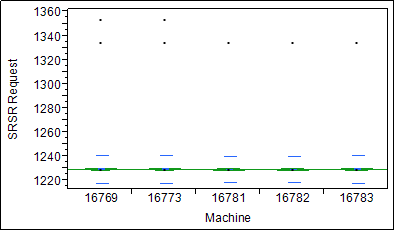
\includegraphics{SRSRRequestMemory.png}
  \caption{Request Memory over 5 machines}
\end{figure}

The results of releasing memory are very similar to that of requesting memory. The mean time taken to release memory is 1229.237ns. The variations among different machines were very small, giving an F Ratio of 0.0328. This shows that the performance is consistent across different hardware. The performance was as well consistent within itself, the fastest machine had a 95\% confidence interval of [1228.5, 1229.9], and for the slowest [1228.6, 1230.0]. Releasing memory takes on average a little under three times as long as requesting memory

\begin{figure}[h!]
  \centering
    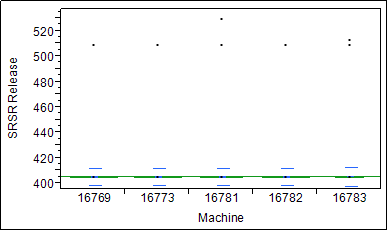
\includegraphics{SRSRReleaseMemory.png}
  \caption{Release Memory over 5 machines}
\end{figure}

\subsection{Cumulative Memory Requests}
\label{sec:cumulative_memory_requests}

\par The cumulative memory requests condition had 50 memory blocks requested and then subsequently released. This differs from experiment in \ref{sec:single_request_single_release} where the requested memory blocks do not accumulate. The purpose of this experiment is to see the effect of depleting resources on run time. Once again, trials were taken over 5 machines, however, each machine showed the same performance. To acheive this, the following two method calls were made.

\begin{algorithm}
  \caption{Cumulative Memory Request and Memory release}
  \begin{algorithmic}[1]
    \Function{Cumulative\_Request}{}
      \For{$i = 0$ to $50$}
        \State RequestStartTime[i] $\gets$ Curent Time
        \State memoryBlock $\gets$  \Call{request\_memory\_block}{}
        \State RequestEndTime[i] $\gets$ Curent Time
      \EndFor
    \EndFunction

    \Function{Cumulative\_Release}{}
      \For{$i = 0$ to $50$}
        \State ReleaseStartTime[i] $\gets$ Curent Time
        \State memoryBlock $\gets$  \Call{release\_memory\_block}{}
        \State ReleaseEndTime[i] $\gets$ Curent Time
      \EndFor
    \EndFunction
  \end{algorithmic}
\end{algorithm}

\par Consistent with the Single Request, Single Release experiment, the first memory block requested took 1229ns. A linear trend line is overlaid on top showing an R2 value of 1 (a perfect trend). The trend shows that for each additional memory block requested, the run time increase by 17ns. This linear trend is in accordance with the implementation of the request memory method which has O(n) complexity described in \ref{sec:request_memory}.

\begin{figure}[h!]
  \centering
    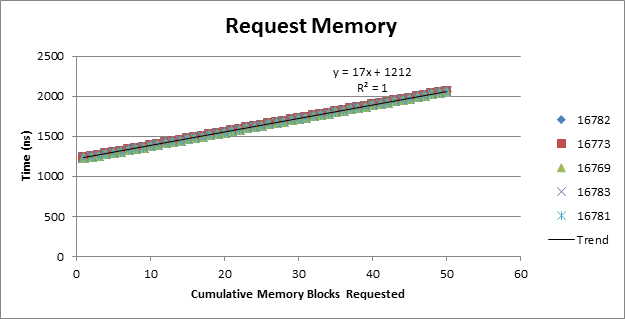
\includegraphics{RequestMemory.png}
  \caption{Release Memory over 5 machines}
\end{figure}

\section{Sending and Receiving Messages}
\subsection{Single Send, Single Receive}
\label{sec:single_send_single_receive}

In this experiment, the send\_message and receive\_message methods were timed. A single message was sent and the time taken was recorded. Similarly, the time taken to receive that message was timed, specifically the time for the function call and not the delay between the time the message was sent and the time the message was received. By doing so we are able to eliminate the effects of having inconsisent memory available (that will be tested in the following experiment). To achieve this, two user processes were defined, the first sends a message of a fixed size then releases the processor, the second would then receive that message and again release the processor. This process would then repeat a total of 498 times. Data was collected across 5 machines, with 498 calls to each function.

\begin{figure}[h!]
  \centering
    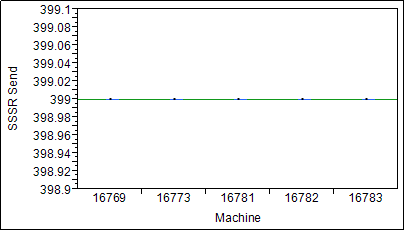
\includegraphics{SSSRSend.png}
    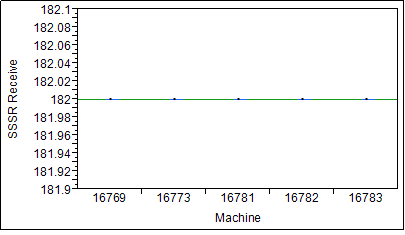
\includegraphics{SSSRReceive.png}
  \caption{Top: Sending messages; Bottom: Receiving messages}
\end{figure}

In this single send, single receive condition, a total of 2490 trials were taken, and the data showed no variation for either sending messages or receiving messages. The mean run time of sending a message is 399ns. Due to the lack of variation on or between each machine this is also the value of the lower and upper bound of the 95\% confidence interval. The same applies for receiving the message, which is twice as fast at 182ns.

\subsection{Cumulative Message Sending}
\label{sec:cumulative_message_sending}

The cumulative message sending condition, as the name implies, had messages accumulate before any were received. The purpose of this is to the see the relation between the number of messages sent (and not yet received) with the time it takes to send a new message. In order to test this, 50 messages were sent from within a single user processes. Once finished, another process would take over and receive those 50 messages. The results from 5 different machines are displayed in the Figure.
\begin{figure}[h!]
  \centering
    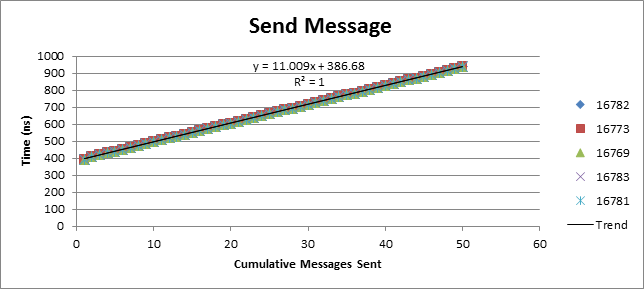
\includegraphics{SendMessage.png}
  \caption{Cumulative message sending}
\end{figure}

Similar to the single send, single receive condition in \ref{sec:single_send_single_receive}, the results were the same across all machines. A linear trend line is superimposed onto the results. The trend displayed has an R2 value of 1 showing that this linear trend is very significant. This correlates with the expected O(n) complexity of the send method described in \ref{sec:send_message}. The trend shows an increase of 11ns per additional message sent.

The message receiving process of this experiment was also measured. For all 250 messages received, the time taken was consistent at 182ns. This is as well expected due to the O(1) complexity of the receive message method describe in \ref{sec:receive_message}.

\subsection{Effects of Message Length}
\label{sec:message_length}
Another factor that was tested is the length of the message being sent. Depending on the implementation for the kernel it is possible that in some cases a longer message will take longer to send or receive. To test this, messages were continuously sent and received in the same manner as the single send, single receive condition in \ref{sec:single_send_single_receive} with the addition of an accumulating message (ie the first message sent was “a”, the second message “aa” and so forth).  This was tested up until a message of 50 characters was sent. As shown in the two figures, the message length had no effect on the time taken to send or receive messages.

\begin{figure}[h!]
  \centering
    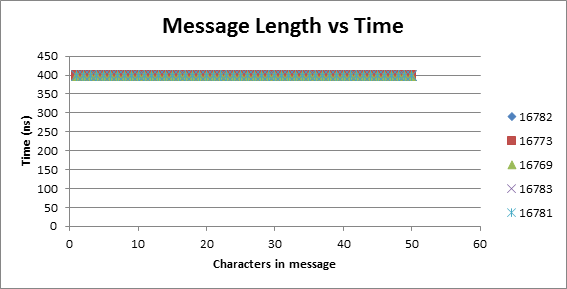
\includegraphics{MessageLength.png}
  \caption{Sending messages with variable message length}
\end{figure}


\appendix
\label{sec:appendix}
\chapter{Memory Layout}
\label{sec:appendix_memory_layout}
\begin{figure}[h]
\setlength{\unitlength}{0.14in} % selecting unit length
\centering % used for centering Figure
\begin{picture}(32,41) % picture environment with the size (dimensions)
 % 32 length units wide, and 15 units high.

\put(-2,43.5) {$0x00000000$}
\put(4.5,44){\vector(1,0){3}}
\put(28,43.5) {Start of Flash}
\put(27.5,44){\vector(-1,0){3}}

\put(8,41){\framebox(16,3){RTX Code}}
\put(8,38){\framebox(16,3){Unmapped Area}}

\put(-2,37.5) {$0x10000000$}
\put(4.5,38){\vector(1,0){3}}
\put(28,37.5) {Start of Ram}
\put(27.5,38){\vector(-1,0){3}}

\put(8,34){\framebox(16,4){RTX Image}}
\put(28,32.5) {End of RTX Image}
\put(27.5,33){\vector(-1,0){3}}

\put(8,33){\framebox(16,1){Padding}}
\put(8,30){\framebox(16,3){PCB 1}}
\put(8,27){\framebox(16,3){PCB 2}}
\put(8,24){\framebox(16,3){PCB ...}}
\put(8,21){\framebox(16,3){PCB n}}
\put(28,20.5) {PCB Allocation End}
\put(27.5,21){\vector(-1,0){3}}

\put(8,15){\framebox(16,6){Heap - Shared by all processes}}

\put(28,14.5) {Stack Allocation End}
\put(27.5,15){\vector(-1,0){3}}
\put(8,12){\framebox(16,3){Process n Stack}}
\put(8,9){\framebox(16,3){Process ... Stack}}
\put(8,6){\framebox(16,3){Process 2 Stack}}
\put(8,3){\framebox(16,3){Process 1 Stack}}

\put(-2,2.5) {$0x10008000$}
\put(4.5,3){\vector(1,0){3}}
\put(28, 2.5) {End of Ram}
\put(27.5, 3){\vector(-1, 0){3}}

\end{picture}
\caption{Layout of Main Memory with n Processes. The RTX Image contains all global and static variables}
\label{fig:memory}
\end{figure}

\chapter{Raw Measurement Data}
\label{appendix:raw_data}

\section{Code Used To Collect Timing Data}
\begin{lstlisting}
static void proc1(void)
{
  timer_test_init();
  static const int memory_block_count = 50;
  static void* memory_blocks[memory_block_count];

  int start_time = 0;
  int end_time = 0;
  LOG("Started single request single release");
  for (int i = 0; i < 1000; i++) {
    start_time = s_test_timer->TC;
    memory_blocks[0] = request_memory_block();
    end_time = s_test_timer->TC;
    LOG("Request: %d", end_time - start_time);
    start_time = s_test_timer->TC;
    release_memory_block(memory_blocks[0]);
    end_time = s_test_timer->TC;
    LOG("Release: %d", end_time - start_time);
  }
  LOG("Finished single request single release");
  LOG("Started requesting");
  for (int i = 0; i < memory_block_count; i++) {
    start_time = s_test_timer->TC;
    memory_blocks[i] = request_memory_block();
    end_time = s_test_timer->TC;
    LOG("%d", end_time - start_time);
  }
  LOG("Finished requesting");
  test_results[REQUEST_MEMORY_TEST] = 1;
  LOG("Started releasing");
  for (int i = 0; i < memory_block_count; i++) {
    start_time = s_test_timer->TC;
    release_memory_block(memory_blocks[i]);
    end_time = s_test_timer->TC;
    LOG("%d", end_time - start_time);
  }
  LOG("Finished releasing");

  test_results[RELEASE_MEMORY_TEST] = 1;
  set_process_priority(1, USER_PROCESS_PRIORITY_LOWEST);
  set_process_priority(2, USER_PROCESS_PRIORITY_HIGH);
  while (1) {
    s_iteration_count++;
    release_processor();
  }
}

//...

static int const required_messages = 50;

static void proc3(void)
{
  LOG("Started receiving messages");
  for (int i = 0; i < required_messages; i++) {
    int start_time = 0;
    int end_time = 0;
    start_time = s_test_timer->TC;
    void* message = receive_message(NULL);
    end_time = s_test_timer->TC;
    LOG("Receive: %d", end_time - start_time);
    release_memory_block(message);
  }
  LOG("Finished receiving messages");
  set_process_priority(5, USER_PROCESS_PRIORITY_HIGH);
  set_process_priority(4, USER_PROCESS_PRIORITY_LOWEST);
  set_process_priority(3, USER_PROCESS_PRIORITY_LOWEST);
  release_processor();
}

static void proc4(void)
{
  LOG("Started sending messages");
  for (int i = 0; i < required_messages; i++) {
    struct msgbuf* message_envelope = (struct msgbuf*)request_memory_block();
    message_envelope->mtype = 10;
    strcpy(message_envelope->mtext, test_phrase);
    int start_time = 0;
    int end_time = 0;
    start_time = s_test_timer->TC;
    send_message(3, message_envelope);
    end_time = s_test_timer->TC;
    LOG("Send: %d", end_time - start_time);
  }
  LOG("Finished sending messages");
  set_process_priority(3, USER_PROCESS_PRIORITY_HIGH);
  set_process_priority(4, USER_PROCESS_PRIORITY_LOWEST);
  release_processor();
}

int sample_size = 500;
static void proc5(void)
{
  set_process_priority(6, USER_PROCESS_PRIORITY_HIGH);
  void* message = receive_message(NULL);
  release_memory_block(message);

  while (true) {
    int start_time = 0;
    int end_time = 0;
    start_time = s_test_timer->TC;
    void* message = receive_message(NULL);
    end_time = s_test_timer->TC;
    LOG("Receive: %d", end_time - start_time);
    release_memory_block(message);
    release_processor();
  }
}

static void proc6(void)
{
  LOG("Started send-receive together");
  for (int i = 0; i < sample_size; i++) {
    struct msgbuf* message_envelope = (struct msgbuf*)request_memory_block();
    message_envelope->mtype = 10;
    strcpy(message_envelope->mtext, test_phrase);
    int start_time = 0;
    int end_time = 0;
    start_time = s_test_timer->TC;
    send_message(5, message_envelope);
    end_time = s_test_timer->TC;
    LOG("Send: %d", end_time - start_time);
    release_processor();
  }
  LOG("Finished send-receive together");

  LOG("Started variable message length together");
  for (int i = 0; i < sample_size; i++) {
    struct msgbuf* message_envelope = (struct msgbuf*)request_memory_block();
    message_envelope->mtype = 10;
    for (int j = 0; j < i; j++) {
      message_envelope->mtext[j] = *"a";
    }
    int start_time = 0;
    int end_time = 0;
    start_time = s_test_timer->TC;
    send_message(5, message_envelope);
    end_time = s_test_timer->TC;
    LOG("Send: %d", end_time - start_time);
    release_processor();
  }
  LOG("Finished variable message length together");
}
\end{lstlisting}
\section{Data Analysis For Single Request Single Release}

\subsection{Request}
Summary of Fit
\newline
\begin{tabular}{l | l}
  Rsquare&2.63E-05 \\
  Adj Rsquare&-0.00077 \\
  Root Mean Square Error&11.43196 \\
  Mean of Response&1229.237 \\
  Observations (or Sum Wgts)&5000 \\
\end{tabular}
\newline

Analysis of Variance
\newline
\begin{tabular}{l | l | l | l | l | l}
Source&DF&Sum of Square&Mean Square&F Ratio&Prob > F \\
\hline
Machine&4&17.14&4.285&0.0328&0.9979 \\
Error&4995&652795.5&130.69&-&- \\
C. Total&4999&652812.7&-&-&- \\
\end{tabular}
\newline

Means of Oneway Anova
\newline
\begin{tabular}{l | l | l | l | l | l}
Machine&Number&Mean&Std Error&Lower 95\%&Upper 95\% \\
\hline
16769&1000&1229.29&0.36151&1228.6&1230 \\
16773&1000&1229.29&0.36151&1228.6&1230 \\
16781&1000&1229.17&0.36151&1228.5&1229.9 \\
16782&1000&1229.17&0.36151&1228.5&1229.9 \\
16783&1000&1229.27&0.36151&1228.6&1230 \\
\end{tabular}
\newline

Means and Std Deviations
\newline
\begin{tabular}{l | l | l | l | l | l | l}
Machine&Number&Mean&Std Dev&Std Err Mean&Lower 95\%&Upper 95\% \\
\hline
16769&1000&1229.29&11.7342&0.37107&1228.6&1230 \\
16773&1000&1229.29&11.7342&0.37107&1228.6&1230 \\
16781&1000&1229.17&11.0616&0.3498&1228.5&1229.9 \\
16782&1000&1229.17&11.0616&0.3498&1228.5&1229.9 \\
16783&1000&1229.27&11.5476&0.36517&1228.6&1230 \\
\end{tabular}
\newline

\subsection{Release}
Summary of Fit
\newline
\begin{tabular}{l | l}
  Rsquare&3.79E-05 \\
  Adj Rsquare&-0.00076 \\
  Root Mean Square Error&6.8087 \\
  Mean of Response&405.4416 \\
  Observations (or Sum Wgts)&5000 \\
\end{tabular}
\newline
  \newline

Analysis of Variance
\newline
\begin{tabular}{l | l | l | l | l | l}
  Source&DF&Sum of Squares&Mean Square&F Ratio&Prob > F \\
  \hline
  Machine&4&8.79&2.1968&0.0474&0.9958 \\
  Error&4995&231560.2&46.3584&-&- \\
  C. Total&4999&231569&-&-&- \\
\end{tabular}
\newline

Means for Oneway Anova
\newline
\begin{tabular}{l | l | l | l | l | l}
  Machine&Number of Trials&Mean&Std Error&Lower 95\%&Upper 95\% \\
  \hline
  16769&1000&405.416&0.21531&404.99&405.84 \\
  16773&1000&405.416&0.21531&404.99&405.84 \\
  16781&1000&405.436&0.21531&405.01&405.86 \\
  16782&1000&405.416&0.21531&404.99&405.84 \\
  16783&1000&405.524&0.21531&405.10&405.95 \\
\end{tabular}
\newline

Means And Std Deviations
\newline
\begin{tabular}{l | l | l | l | l | l |l}
  Machine&Number&Mean&Std Dev&Std Err Mean&Lower 95\%&Upper 95\% \\
  \hline
  16769&1000&405.416&6.56765&0.20769&405.01&405.82 \\
  16773&1000&405.416&6.56765&0.20769&405.01&405.82 \\
  16781&1000&405.436&6.90519&0.21836&405.01&405.86 \\
  16782&1000&405.416&6.56765&0.20769&405.01&405.82 \\
  16783&1000&405.524&7.39649&0.23390&405.07&405.98 \\
\end{tabular}
\newline

\section{Data Analysis for Single Send Single Receive}
\subsection{Send}
Summary of Fit
\newline
\begin{tabular}{l | l}
  Rsquare&- \\
  Adj Rsquare&- \\
  Root Mean Square Error&0 \\
  Mean of Response&399 \\
  Observations (or Sum Wgts)&2490 \\
\end{tabular}
\newline

Analysis of Variance
\newline
\begin{tabular}{l | l | l | l | l | l}
Source&DF&Sum of Square&Mean Square&F Ratio&Prob > F \\
\hline
Machine&4&0&0&-&- \\
Error&2485&0&0&-&- \\
C. Total&2489&0&-&-&- \\
\end{tabular}
\newline

Means of Oneway Anova
\newline
\begin{tabular}{l | l | l | l | l | l}
Machine&Number&Mean&Std Error&Lower 95\%&Upper 95\% \\
\hline
16769&498&399&0&399&399 \\
16773&498&399&0&399&399 \\
16781&498&399&0&399&399 \\
16782&498&399&0&399&399 \\
16783&498&399&0&399&399 \\
\end{tabular}
\newline

Means and Std Deviations
\newline
\begin{tabular}{l | l | l | l | l | l | l}
Machine&Number&Mean&Std Dev&Std Err Mean&Lower 95\%&Upper 95\% \\
\hline
16769&498&399&0&0&399&399 \\
16773&498&399&0&0&399&399 \\
16781&498&399&0&0&399&399 \\
16782&498&399&0&0&399&399 \\
16783&498&399&0&0&399&399 \\
\end{tabular}
\newline

\subsection{Receive}
Summary of Fit
\newline
\begin{tabular}{l | l}
  Rsquare&- \\
  Adj Rsquare&- \\
  Root Mean Square Error&0 \\
  Mean of Response&182 \\
  Observations (or Sum Wgts)&2490 \\
\end{tabular}
\newline

Analysis of Variance
\newline
\begin{tabular}{l | l | l | l | l | l}
Source&DF&Sum of Square&Mean Square&F Ratio&Prob > F \\
\hline
Machine&4&0&0&-&- \\
Error&2485&0&0&-&- \\
C. Total&2489&0&-&-&- \\
\end{tabular}
\newline

Means of Oneway Anova
\newline
\begin{tabular}{l | l | l | l | l | l}
Machine&Number&Mean&Std Error&Lower 95\%&Upper 95\% \\
\hline
16769&498&182&0&182&182 \\
16773&498&182&0&182&182 \\
16781&498&182&0&182&182 \\
16782&498&182&0&182&182 \\
16783&498&182&0&182&182 \\
\end{tabular}
\newline

Means and Std Deviations
\newline
\begin{tabular}{l | l | l | l | l | l | l}
Machine&Number&Mean&Std Dev&Std Err Mean&Lower 95\%&Upper 95\% \\
\hline
16769&498&182&0&0&182&182 \\
16773&498&182&0&0&182&182 \\
16781&498&182&0&0&182&182 \\
16782&498&182&0&0&182&182 \\
16783&498&182&0&0&182&182 \\
\end{tabular}
\newline

\end{document}
